\documentclass[times, utf8, seminar]{fit}

%\batchmode
%\usepackage{booktabs}
\usepackage{listings}
\usepackage{longtable}
\usepackage{xcolor}
\usepackage{float}
\usepackage{enumitem}
\usepackage{hyperref}
\usepackage{enumerate}
\usepackage{graphicx}
\usepackage{etoolbox}

\begin{document}

\title{Projekat: Unapređenje informacionog sistema na primjeru jedne kompanije}

\author{Ernad Husremović}
\brindex{DL 2792}
\verzija {1.0.0}

\mentor{prof.dr Murat Prašo}

\maketitle

\tableofcontents

\listoftables
\listoffigures

% abstract begin
\begin{sazetak}


Sažetak na bosanskom jeziku.

\kljucnerijeci{bosanska rijec 1, bosanska rijec 2}
\end{sazetak}

\engtitle{Naslov na engleskom jeziku}
\begin{abstract}
Abstract na engleskom jeziku.

\keywords{key1, key2, key3}
\end{abstract}

% abstract end

\chapter{Uvod}

\section{Legalizacija - bezpovratne promjene na IT tržištu BiH}

Akcije državnih inspekcijskih organa na suzbijanju nelegalnog softvera (nadalje legalizacija) sa početkom 2012 godine označila je početak krupnih promjena na tržištu informatičkih \engl{information technology, nadalje IT} rješenja u Bosni i Hercegovini. 
Većina poslovnih subjekata koja se u proteklim godinama opremila "jeftinim" nelegalnim softverom \engl{software} našla se u nezavidnoj situaciji.
Usljed visokih troškovima legalizacije "Microsoft" softvera\footnote{familija "Microsoft Windows" OS-ova, uz svuda prisutni ali i redovno nelegalno instalirani "Microsoft Office" uredski paket}, pojavila se potražnja za softverom drugih proizvođača.  

\section{OSS softver}

Preduzeće "bring.out"\footnote{\url{http://www.bring.out.ba/}} je dugi niz godina orjentisano na ponudu sistema baziranih na softveru otvorenog koda \engl{open source software, nadalje OSS}.

Potražnja za Linux/Ubuntu serverskim rješenjima \footnote{\url{http://linux.com}, \url{http://ubuntu.com}}) je postojala i prije legalizacije. Međutim, tek nakon legalizacije pojavila se potražnja za cjelovitim informatičkim IT rješenjima baziranim na OSS-u:
\begin{itemize}
  \item server operativni sistem (nadalje OS)
  \item desktop operativni sistem
  \item aplikativni softver
  \begin{itemize}
    \item opći softver za uredske potrebe
    \item poslovni softver za podršku tekućim operacijama kompanije \engl{Enterprise Resource Planning, nadalje ERP}
  \end{itemize}
\end{itemize}

\subsection{Ubuntu Linux}
"Ubuntu" Linux distribucija radi svoje jednostavnosti i kvaliteta postao popularan desktop OS.

Za razliku od "Windows" operativnih sistema, "Ubuntu" desktop sistem sadrži kompletan set aplikacija za svakodnevne potrebe:
\begin{itemize}
  \item LibreOffice uredski paket za pravljenje tekstualnih i tabelarnih dokumenata, prezentacija i crteža\footnote{U funkcionalnom smislu sličan "Microsoft office" setu aplikacija. Može obrađivati većinu "Microsoft office" dokumenata}
  \item "Inkscape", program za vektorsku grafiku \cite{inkscape}
  \item "GIMP", program za bitmapiranu grafiku
  \item "Evince", preglednik PDF dokumenata
  \item "Firefox", "Chromium" internet pretraživači
  \item "OpenProj", program za izradu i praćenje projekata\footnote{U funkcionalnom smislu sličan "Microsoft project" aplikaciji}
\end{itemize}  

 
\subsection{Razlike između otvorenog i zatvorenog softvera} 

S obzirom da su za ovaj projekat najbitniji fokus poređenja će biti "Windows" i "Ubuntu" OS. 

Lista iz predhodne sekcije predstavlja djelimičnu listu dostupnih aplikacija. Međutim, i to je dovoljno da se uoči bitna razlika između "Windows" i "Ubuntu" OS-a. 

Uz "Windows" se isporučuje samo operativni sistem, dok "Ubuntu" kao i ostale linux distribucije isporučuju kompletan sistem koji korisnik može odmah početi koristiti.

U ranom stadiju razvoja OSS softver je manjkao sa kvalitetnom dokumentacijom. Sada to nije slučaj. 

Razvoj "open source" softvera je suštinski drugačiji u odnosu na razvoj zatvorenog sofvera. Kod zatvorenog softvera sve ključne razvojne aktivnosti i sudbina softvera nalaze se u rukama jednog proizvođača.

Kod OSS-a postoji velika uključenost zajednice korisnika \engl{community}, što omogućava da se sve komponente softvera razvijaju u skladu sa potrebama i zahtjevima zajednice. Korisnicima je na raspolaganju velika količina dokumentacije koja se takođe razvija na principima otvorenosti.

Korisik ubuntu sistema na raspolaganju ima odličnu dokumentaciju za serverske \cite{ubuntudesktop} i desktop \cite{ubuntuserver}.

Zahvaljujući otvorenosti, lokalizacija programa i korisničke dokumentacije (prevod i prilagodbe za lokalno tržipte) za OSS nije vođena samo komercijalnim motivima. U mnogim zemljama postoje jake zajednice korisnika koje lokalizaciju "open source" softvera vrše na bazi volonterizma. Kako se radi o projektima od velikog javnog značaja, te zajednice su često finansirane od strane države.

Svijetli primjeri država u regionu kojima postoje jake zajednice FOSS \engl{Free and open source software} i OSS  korisnika su Makedonija i Slovenija.

Na žalost, Bosna i Hercegovina, kao i u većini stvari, na tom planu zaostaje. 

\subsection{"F18 knowhowERP" softver}
Pored standardnih komponentni "Ubuntu" OS-a, za ERP softver će se koristiti "F18" knowhowERP software.

"F18" knowhowERP\footnote{\url{http://redmine.bring.out.ba/projects/f18}} je multiplatformsko "open source" ERP rješenje, proizvod firme "bring.out".  

Predhodnik "F18" je programsko rješenje "FMK" koje se na lokalnom tržištu koristi od 1994 godine.

"F18" je softver pravljena od Bosanaca za BiH tržište. "F18" je u cjelosti domaći proizvod.

\subsection{Cjelovito OSS IT rješenje}
Na osnovu svega što je do sada izloženo, bosanskom klijentu je moguće ponuditi cjelovito OSS IT rješenje.  

Ovaj projekat će obuhvatiti instalaciju jednog takvog sistema kod klijenta.

\section{Profil korisnika projekta}
Korisnik je mala kompanija koja se bavi trgovinom. Sa stanovišta IT-a kompanija se sastoji od:
\begin{itemize}
  \item maloprodajna mreža od 5 prodavnica
  \item centrala kompanije sa knjigovodstvom, 4 radne stanice
  \item 1 server baze podataka 
\end{itemize}

\chapter{Analiza}

\section{Analiza problema}

Povod klijentu za traženje novog rješenja je nedavna akcija legalizacije. 

Međutim, analiza je pokazala da su glavni problemi leže u činjenici da postojeći poslovni IS ne obezbjeđuje sve potrebne podatke. Već nakon prvog sastanka sa klijentom utvrđeni su sljedeći problemi, prikazani piramidom problema (\cite{prasopro}):

\begin{figure}[H]
\centering
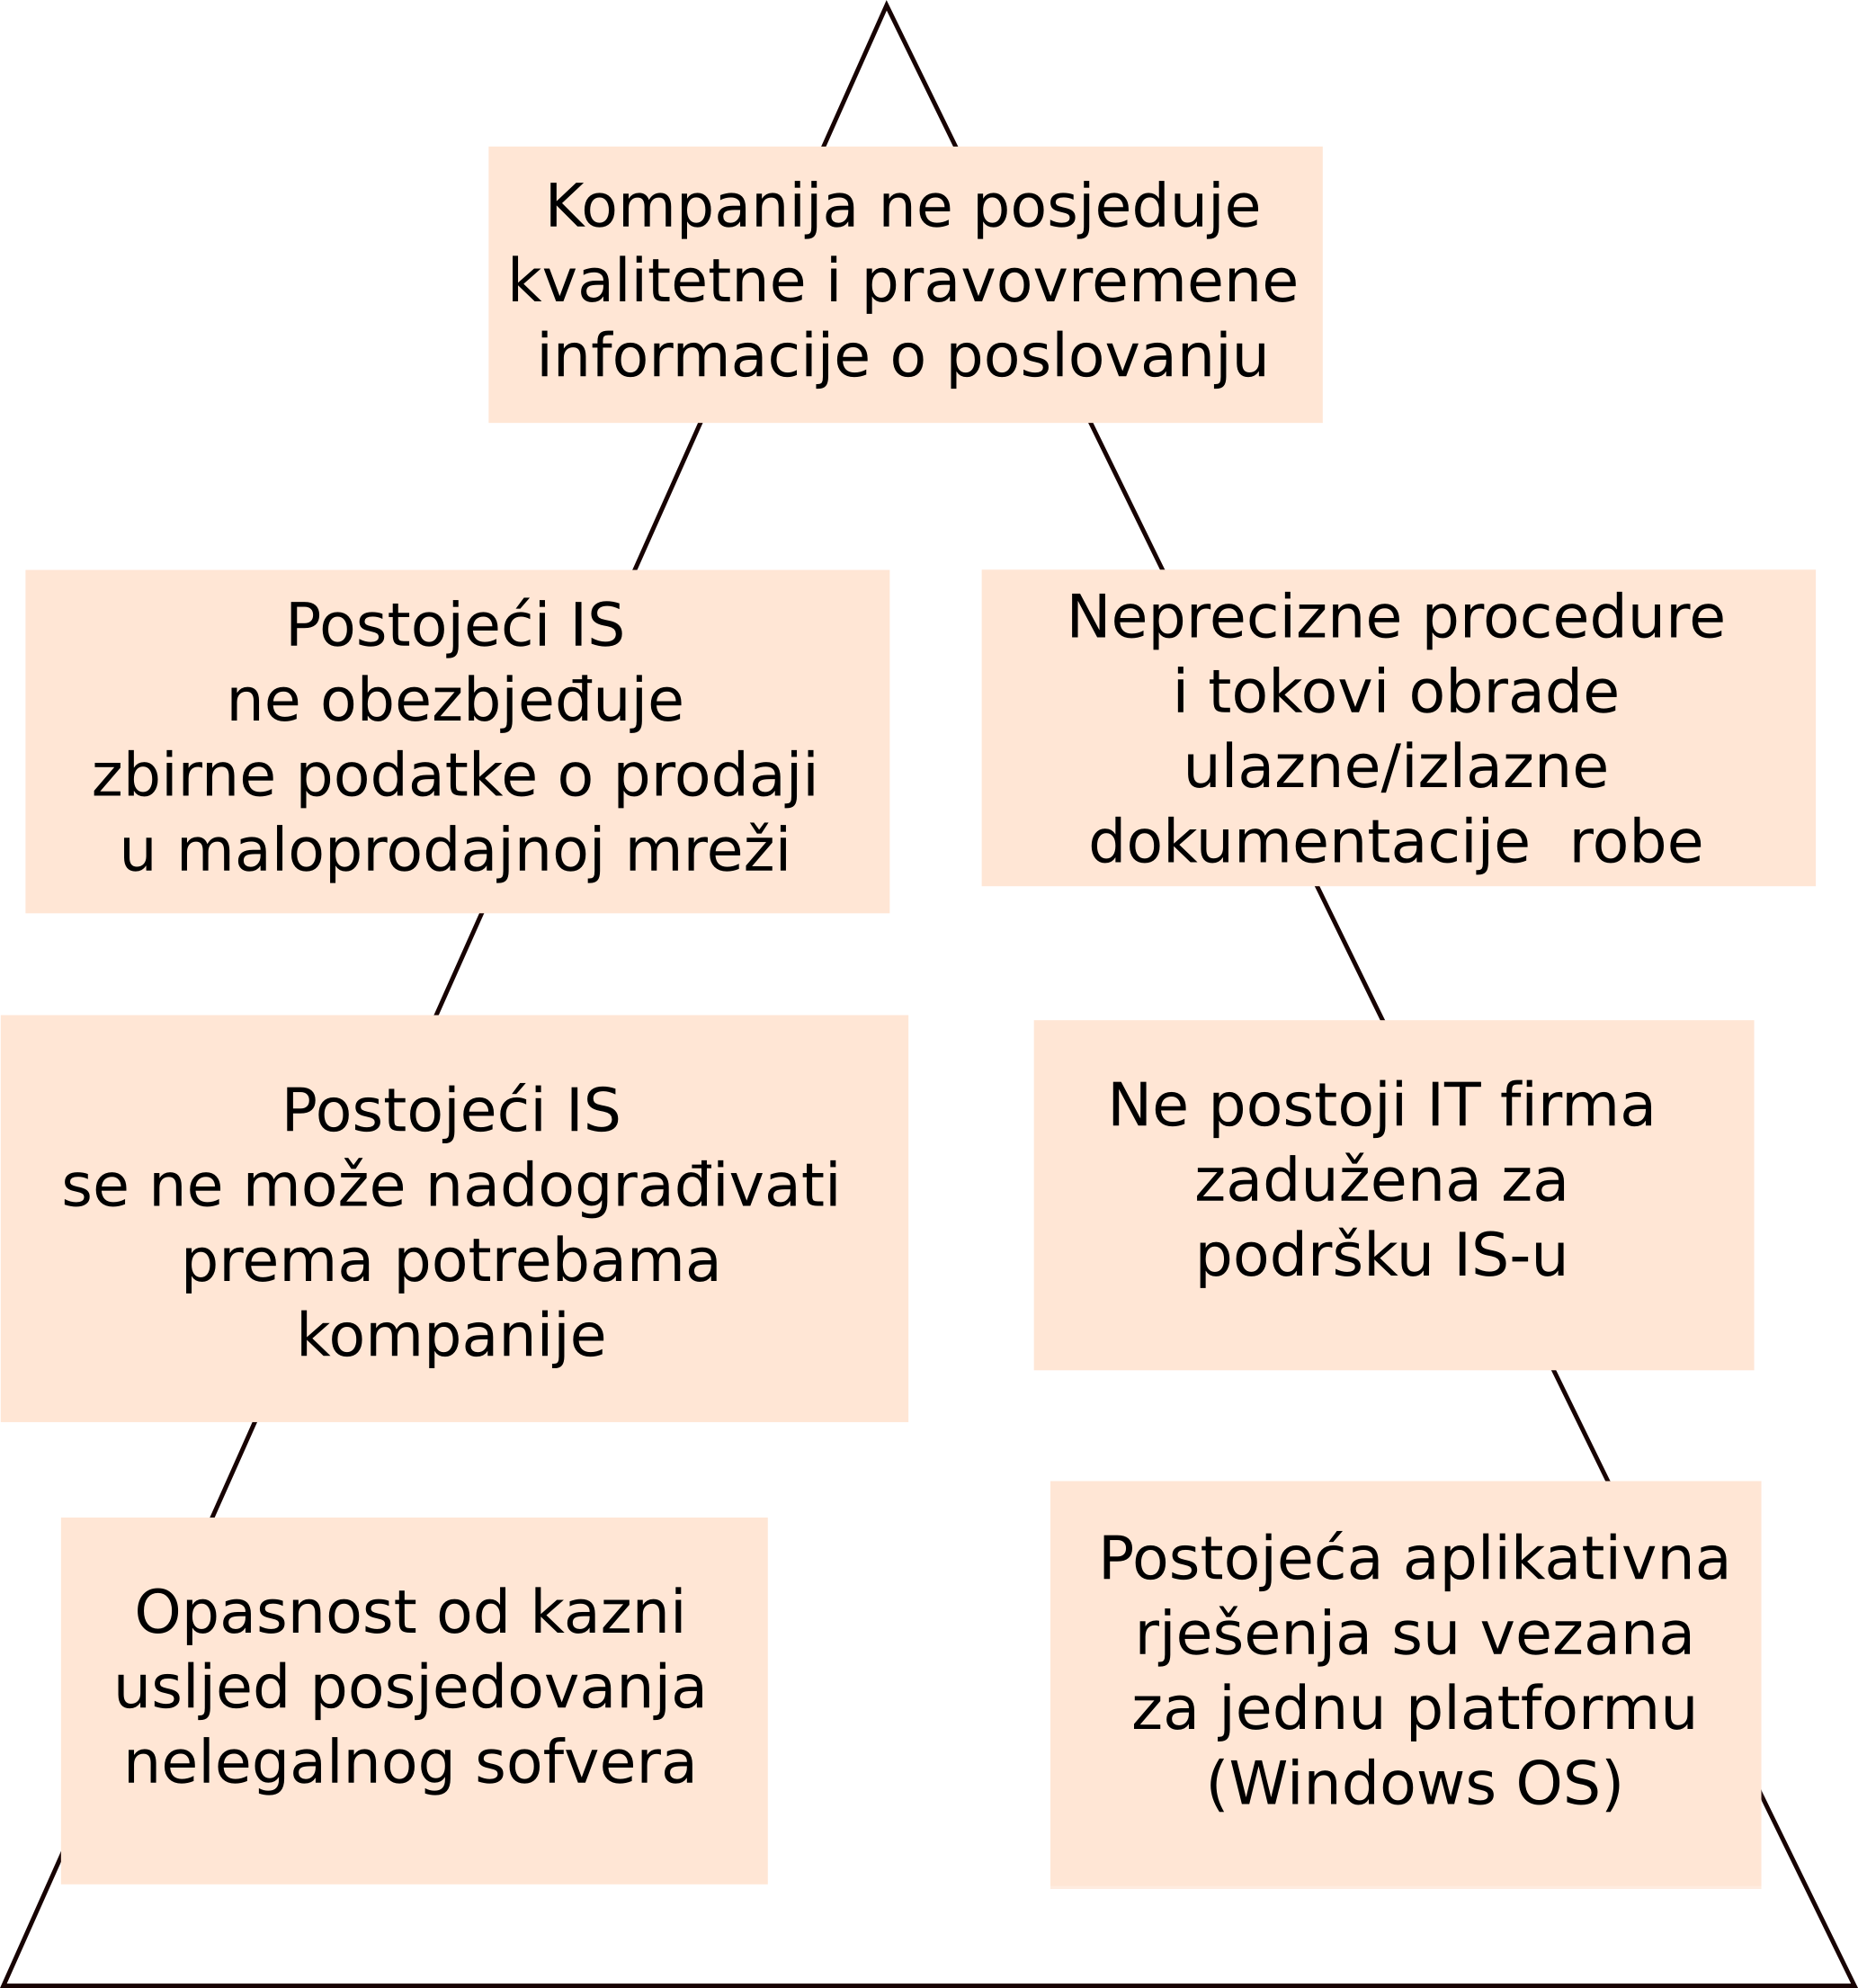
\includegraphics[width=12cm]{img/piramida_problema.png}
\caption{Piramida problema}
%\caption{bla bla (\cite{web:eric})}
\end{figure}

Piramida na vrhu prikazuje opće probleme da bi se idući ka dnu ti problemi konkretizirali.  

\section{Analiza cilja}
Analizom problema prezentovanih piramidom problema brzo dolazimo do strateškog cilja ovog projekta:
%\patchcmd{\quote}{\rightmargin}{\leftmargin 6em \rightmargin}{}{}
\begin{quote}
\em Uvođenjem novog IS-a poboljšati pravovremenost i kvalitet tekućih informacija o poslovanju.} 
\end{quote}
Analogno ranijem grafičkom prikazu problema, putem piramide ciljeva od dna ka vrhu prezentujemo ciljeve čijom realizacijom postižemo strateški cilj:

\begin{figure}[H]
\centering
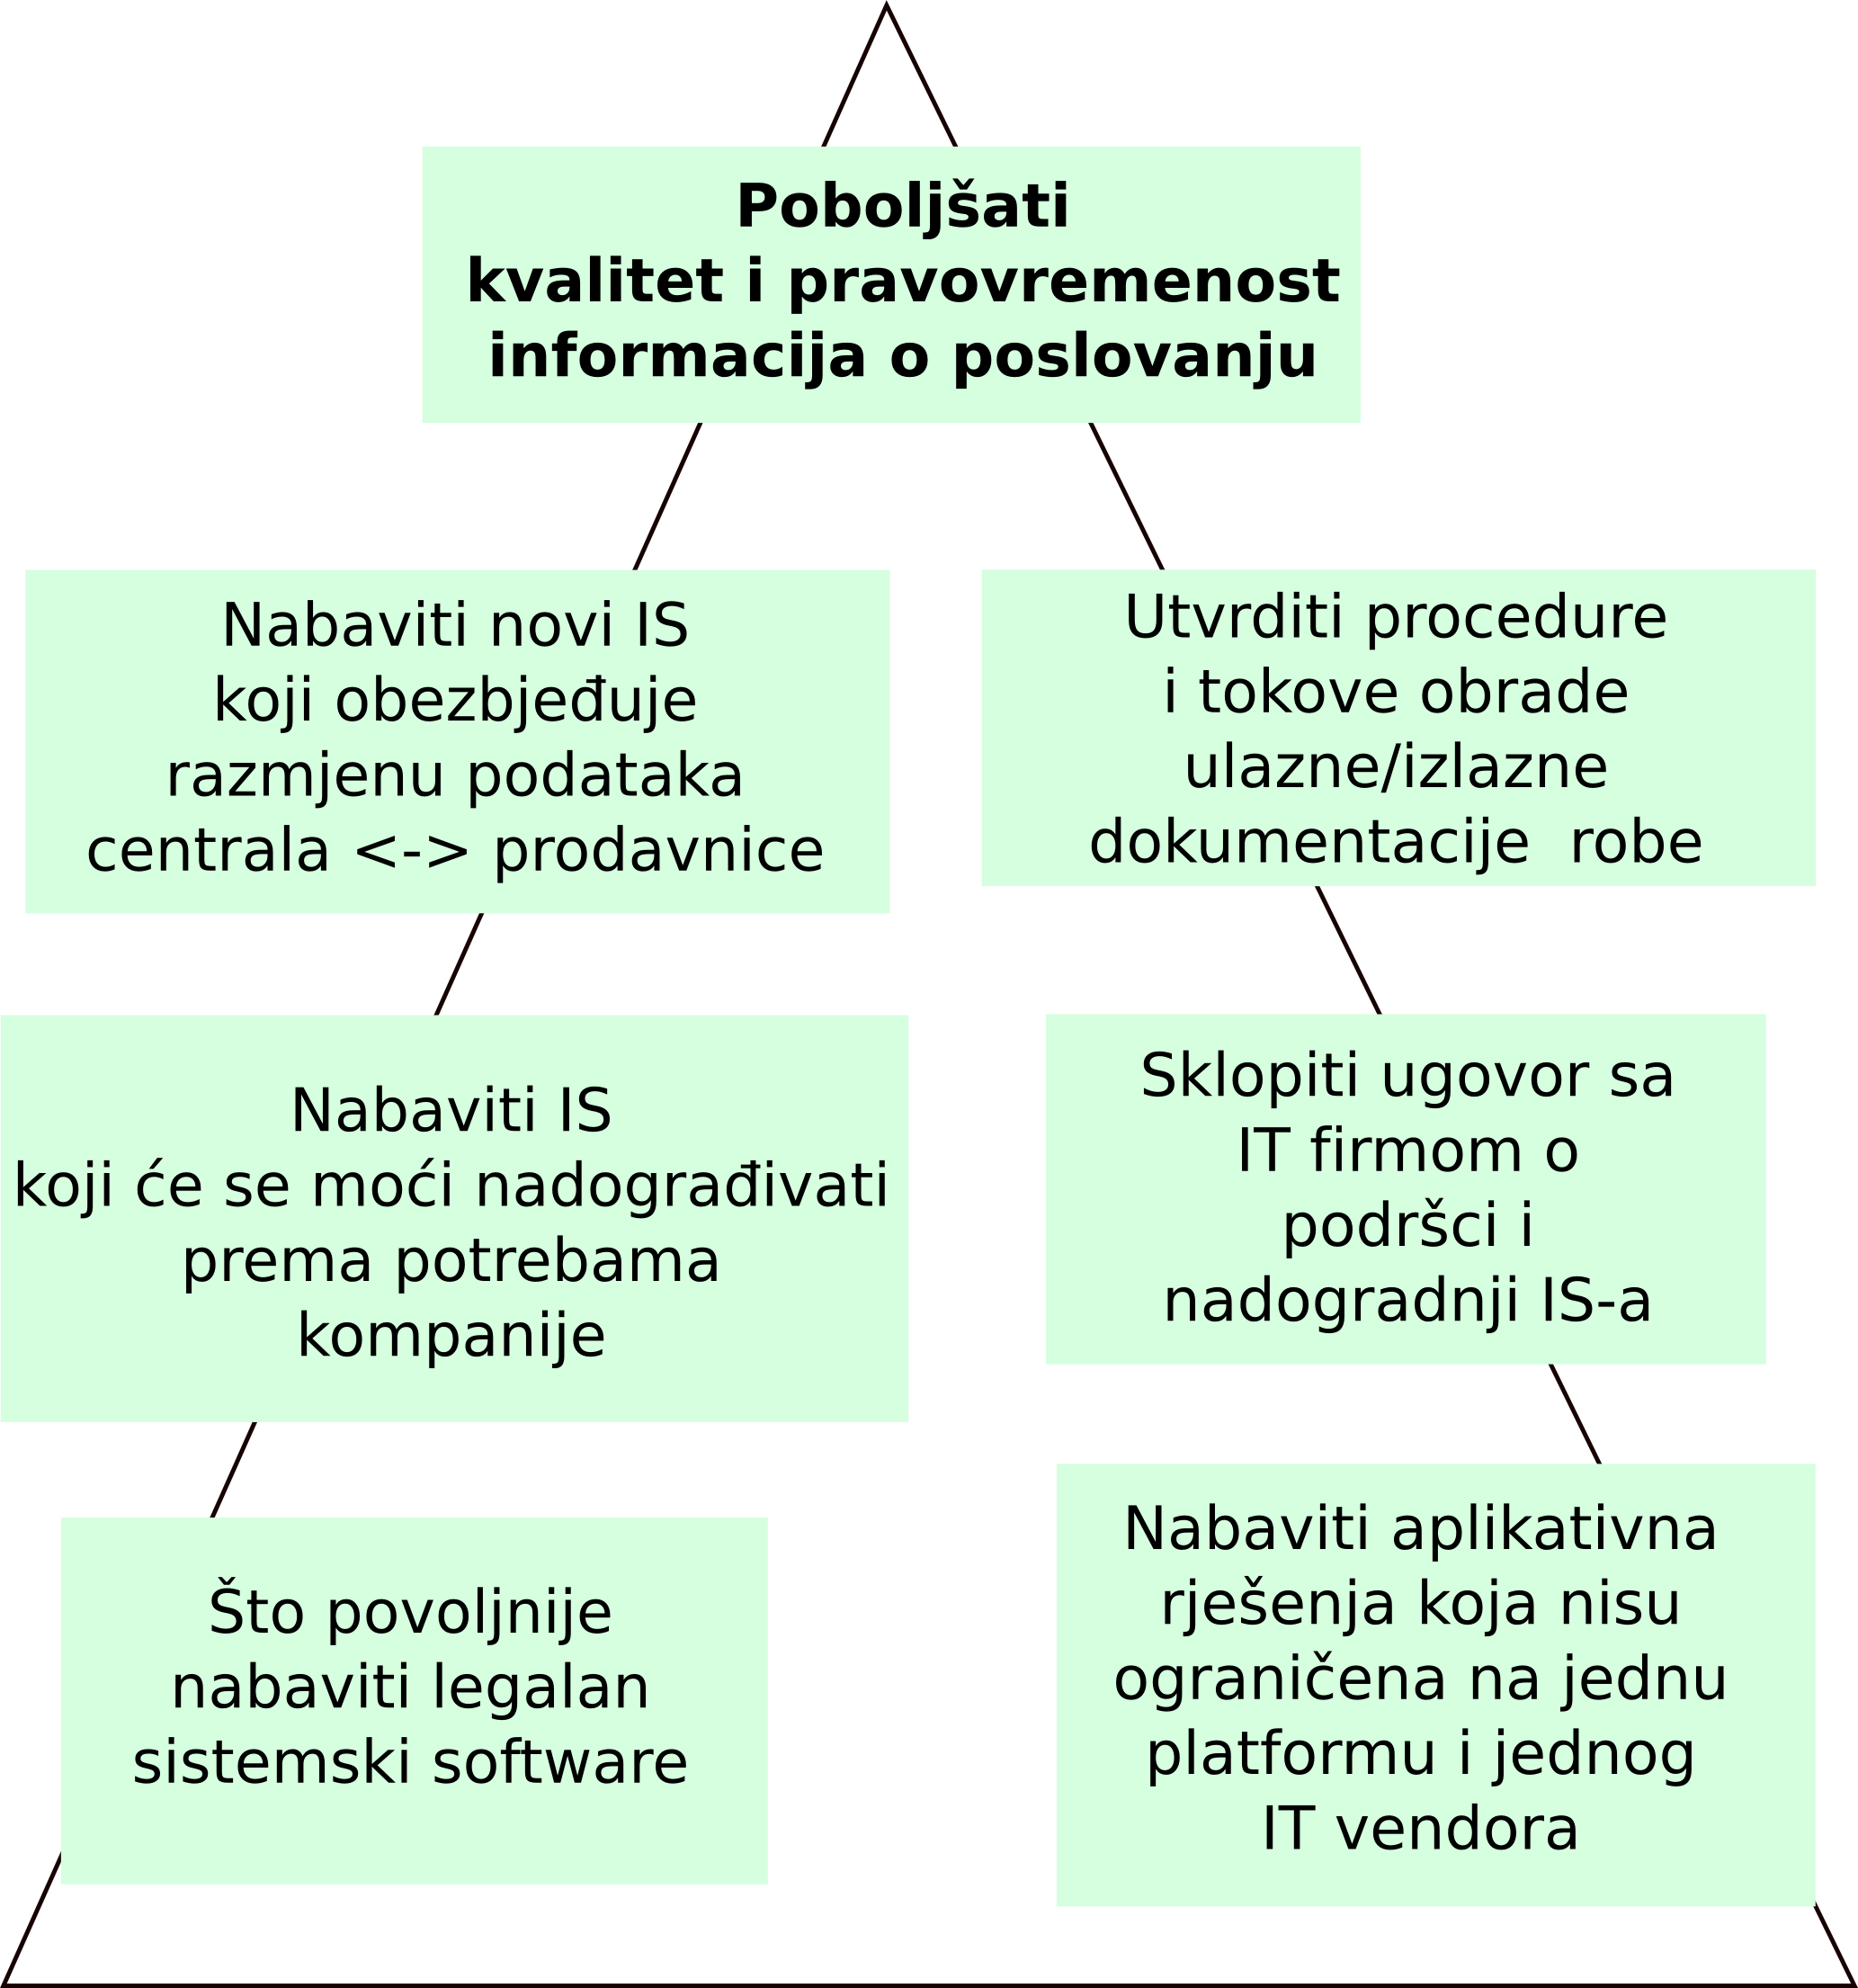
\includegraphics[width=12cm]{img/piramida_cilja.png}
\caption{Piramida cilja}
\end{figure}

\section{Logički okvir projekta}
Na kraju analize dolazimo do ključnih odrednica projekta:
\begin{table}[h]
%\centering
\resizebox{15cm}{!} {
\begin{tabular}{ | r | l | }
\hline
Svrha projekta: & Unapređenje poslovanja kompanije obezbjeđenjem kvalitetnijih informacija o poslovanju \\ \hline
Cilj: & Uvođenje novog informacionog sistema \\ \hline
Ulazi projekta: & Postojeći informacioni sistem, postojeća organizacija poslovanja \\ \hline
Izlazi projekta: & Unapređeni informacioni sistem, unapređena organizacija poslovanja \\ \hline
\end{tabular}
}

\caption{Logički okvir projekta}
\end{table}


\chapter{Upravljanje projektom}

Kvalitetno upravljanje projektom zahtjeva cjelovid uvid u projekat.  

Upravljanje podrazumjeva uvid i praćenje svih bitnih aspekata projekta:
\begin{itemize}
  \item tehničkih
  \item vremenskih
  \item angažovanje ljudskih i materijalnih resursa
  \item finansijskih
\end{itemize}

\pagebreak
\section{Tehnički aspekti}

U uvodnom dijelu su prezentovane tehnologije koje će se koristiti za izgradnji IS-a. Zato taj dio nećemo ponavljati ovdje.

Uspješno upravljanje projektom traži identifikaciju i kvantifikaciju rizika, te planiranje odgovora na pojedinačne rizike.

\subsection{Glavni rizici projekta}

\begin{table}[!h]
\centering
\begin{tabular}{ |p{1.5cm}|p{4cm}|p{7.5cm}|p{1.5cm}| }
\hline
Oznaka & Rizik & Opis & Prioritet  \\ \hline\hline
R1 & Promjena navika kod korisnika & Novi IS pretpostavlja radikalno zamjenu softvera: od desktopa do ERP rješenja & Visok \\ \hline
R2 & bring.out je jedini OSS IT vendor na bosanskom tržištu & Iako su tehnologije koje se implementiraju otvorene, na BH tržištu ne postoje drugi vendori koji nude slična rješenja & Visok \\ \hline
R3 & Nemar države za non-Windows sisteme & Državne institucije podrazumjevaju da porezni obveznici posjeduju Windows OS & Visok \\ \hline
R4 & Ponuđeno ERP rješenje neće zadovoljiti potrebe klijenta & Opasnost da će klijent F18 knowhow ERP percipirati kao neadekvatno ERP rješenje & Srednji \\ \hline
R5 & Neredovno finansiranje projekta & Klijent neće moći obezbjediti redovno finansiranje projekta iz tekućih izvora & Srednji \\ \hline
\end{tabular}
\caption{Lista rizika}
\end{table}

\subsection{Strategija odgovora na pojedinačne rizike} 

U sljedećoj tabeli dajemo prikaz preventivnih i akcija kontrole za identificirane rizike:

\begin{table}[!h]
\centering
\begin{tabular}{|p{1.7cm}|p{13.2cm}|}
\hline
Oznaka & Preventivne i kontrolne akcije  \\ \hline\hline
R1 & Veću pažnju posvetiti obuci korisnika \\ \hline
R2 & Otvorenim pristupom klijentu pokazati da odnose sa klijentom ne gradi na bazi monopola, nego upravo suprotnoe. Stalna komunikacija sa klijentom je najbolji način da se otkloni bojazan klijetna po ovom pitanju\\ \hline
R3 & Aktivnim djelovanjem prema državnim institucijama obezbjediti "bring.out" treba obezbjediti da njegovi klijenti ne budu korisnici drugog reda zato što ne koriste "Windows OS"\\ \hline 
R4 & Softver je alat. Koliko god on dobar bio, on sam neće uraditi posao. IT vendor se treba aktivno uključiti u probleme i potrebe korisnika, pomoći mu da organizuje poslovanje u skladu sa potrebama i glavnim ciljevima IS-a.\\ \hline
R5 & U slučaju objektivnih problema, dogovorom prilagoditi dinamiku plaćanja. S obzirom da se u cjelini radi o sopstvenim proizvodima, IT vendor ima mogućnost učiniti ovakve ustupke klijentu. \\ \hline
\end{tabular}
\caption{Kontrola rizika}
\end{table}

\pagebreak
\section{Vremenski aspekti}

Dinamika realizacije projekta je utvrđena tokom preliminarnih razgovora sa klijentom. Kao okvirno vrijeme dogovoren je 1 mjesec za realizaciju uz dodatnih 2-3 mjeseca označenih kao period stabilizacije sistema. 

Napravljeni dinamički plan je ispoštovao okvire tog dogovora:

\begin{table}[!h]
\centering
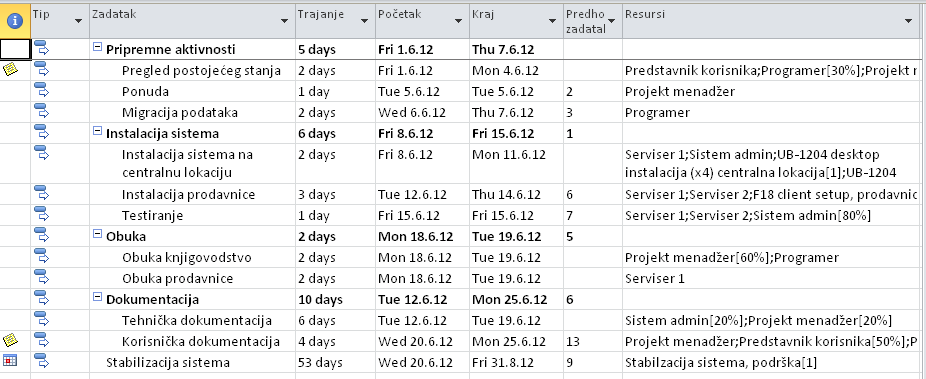
\includegraphics[width=15.5cm]{img/dinamika_sheet.png}
\caption{Tabelarni pregled projektnih zadataka}
\end{table}

Kao nastavak tabelarnom pregledu slijedi gantogram:

\begin{figure}[!h]
\centering
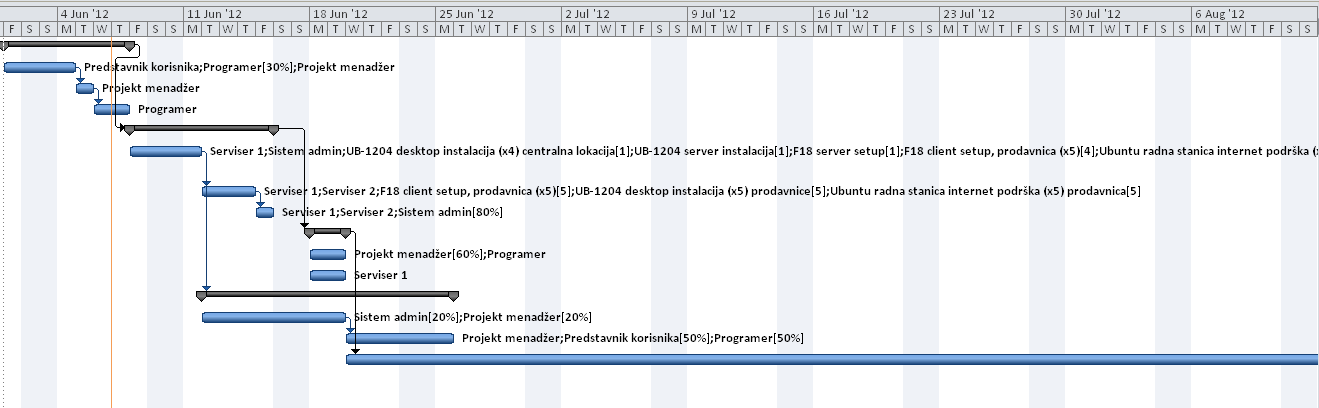
\includegraphics[width=15.5cm]{img/dinamika_gant.png}
\caption{Gantogram projekta}
\end{figure}

Vrijeme realizacije je \textbf{3 mjeseca}, period realizacije \textbf{01.06.2012 - 31.08.2012}. 

\pagebreak
\section{Resursi}
\subsection{Materijalni resursi}
Pregled materijalnih resursa:
\begin{table}[h]
\centering
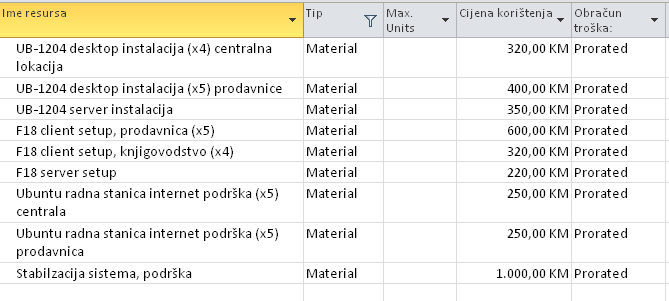
\includegraphics[width=15cm]{img/materijalni_resursi.png}
\caption{Pregled materijalnih resursa}
\end{table}

Treba naglasiti da se u slučaju "open source" sofvera ne radi o "klasičnim" materijanim resursima. Kod OSS-a prodaja licenci za korištenje kao troškovna stavka ne postoji. Klijent plaća instalaciju i podešenje sistema davaocu IT usluga \engl{IT vendor, IT provider}.

S obzirom da su cijene tih usluga normirane, te usluge je najpogodnije u projektu izraziti kao materijalne resurse.

Posebna stavka je "Stabilizacija sistema, podrška". Ova stavka predstavlja iznos ugovora o podršci u periodu stabilizacije sistema koji traje cca 2-3 mjeseca.

U tom periodu se očekuju intenzivne aktivnosti servisnog i programerskog tima na rješavanju zahtjeva novog korisnika.

Iako bi se moglo reći da ova stavka pripada periodu eksplotacije projekta, mi smo se radi preglednosti i dogovorene dinamike plaćanja uvrstili unutar realizacije projekta.

Zato je zadatku "Stabilizacija" u projektnom planu alociran samo ovaj materijalni resurs.

Sveukupno, podjelu na radne i materijalne resurse treba uzeti uslovno. Ovakva podjela je napravljena radi preglednosti i kalkulacije troškova projekta.  

\subsection{Ljudski resursi}
Pregled ljudskih resursa (projektni tim) potrebnih za realizaciju projekta:

\begin{table}[!h]
\centering
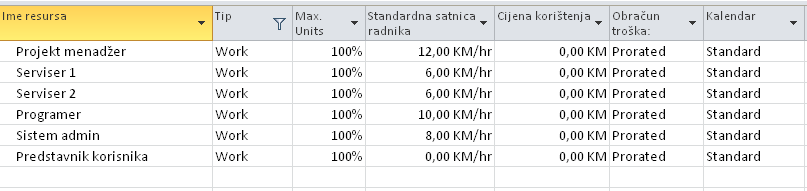
\includegraphics[width=15.5cm]{img/ljudski_resursi.png}
\caption{Pregled ljudskih resursa}
\end{table}

Raspored tima tokom realizacije projekta:

\begin{figure}[!h]
\centering
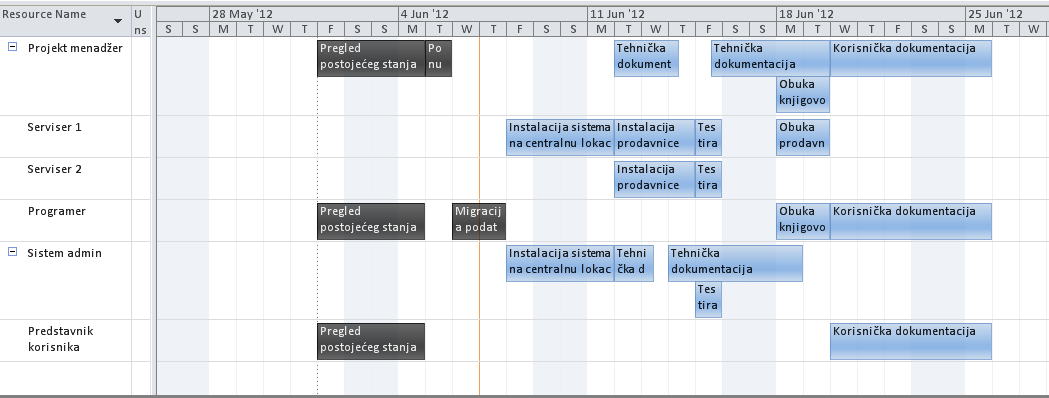
\includegraphics[width=15.5cm]{img/team_planner.png}
\caption{Pregled alokacije ljudskih resursa}
\end{figure}

Radi planiranja sastanaka uvršten je predstavnik klijenta. Zbog pravilne kalkulacije troškova sa stanovišta klijenta, troškovi predstavnika su 0 KM/h.

\pagebreak
\section{Finansijski aspekti}
\subsection{Budžet projekta}
\begin{table}[!h]
\centering
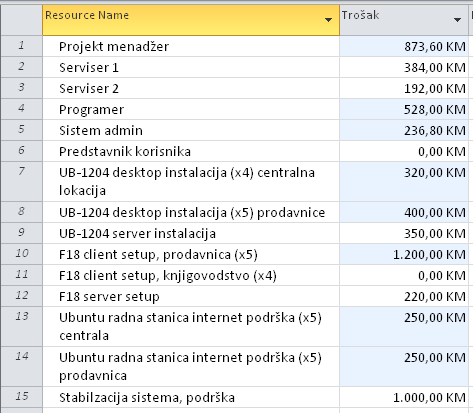
\includegraphics[height=7cm]{img/troskovi.png}
\caption{Pregled ukupnih troškova angažovanja resursa}
\end{table}

Ukupni troškovi realizacije projekta, uključujući fazu stabilizacije su \textbf{6204,40 KM}.

Navedeni su iznosi neto, bez uračnotog PDV-a.

\subsection{Finansiranje projekta}

Prodavac i klijent su dogovorili sjedeću dinamiku plaćanja:

\begin{table}[h]
\centering
\resizebox{15cm}{!} {
\begin{tabular}{ | r | c | c | r | }
\hline
Pozicija & preduslov za plaćanje & Vrijeme & Iznos (KM) bez PDV \\ \hline\hline
Avans: & - & 01.06.2012 & 2000 \\ \hline
Instalacija: & po okončanoj instalaciji & 01.07.2012 & 2000 \\ \hline
stabilizacija 1 & aktivna podrška klijentu & 01.08.2012 & 1000 \\ \hline 
stabilizacija 2 & aktivna podrška klijentu & 31.08.2012 & 1204.40 \\ \hline\hline 
                &                          &    UKUPNO: & 6204.40 \\ \hline
\end{tabular}
}
\caption{Dinamika plaćanja}
\end{table}

Ova dinamika omogućava klijentu da iz sopstvenih izvora (tekućih operativnih prihoda poslovanja \cite{prasorep}) finansira projekat.

\subsection{Ocjena opravdanosti investicije}

Analizu opravdanosti investicije baziraćemo na bazi alternativnog rješenja u kome korisnik jedino plaća troškove legalizacije postojećeg sistemskog sofvera.
Znači danećemo u kalkulaciju staviti troškove legalizacije uredskog "Microsoft office" softvera, niti nabavku novog ERP rješenja.

Kada bi se te stavke uvrstile u kalkulaciju opravdanosti, interna stopa rentabilnosti bi bila puno veća.

Međutim, čak i u ovom konzervativnom scenariju troškova, naš projekat ima visoku internu stopu rentabilnosti od \textbf{36,9\%}, što nam sljedeća kalkulacija pokazuje:

\begin{table}[!h]
\centering
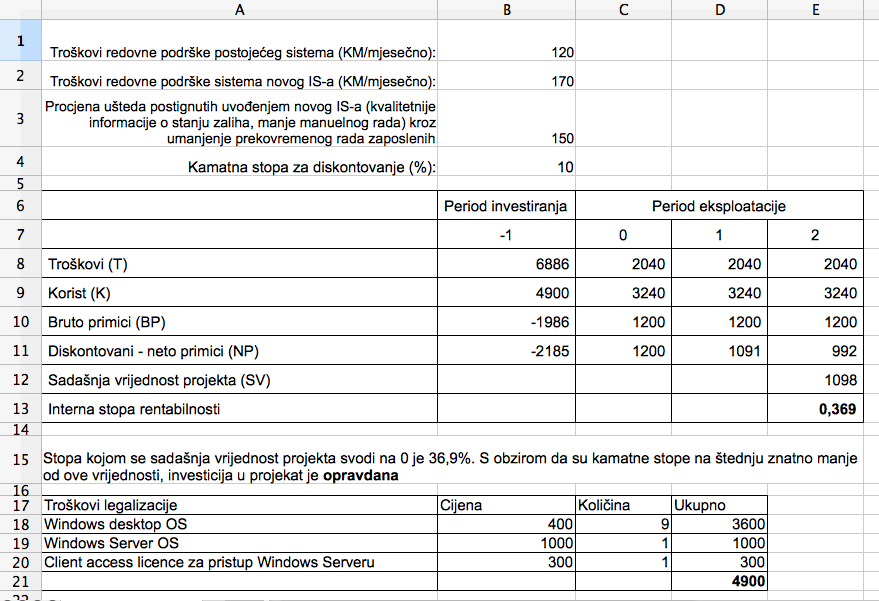
\includegraphics[height=10cm]{img/kalk_opravdanost.png}
\caption{Kalkulacija opravdanosti investicije}
\end{table}

\chapter{Zaključak}

Finansijski indikatori iz prethodnog poglavlja jasno kazuju da je predloženo IT rješenja bazirano na otvorenim tehnologijama u finansijskom smislu isplativa opcija.

Troškovi licenci IS-a koji je izgrađen za zatvorenom - vlasničkom softveru \engl{proprietary software} su tako veliki, da će većina bosanskih poslovnih korisnika na licence potrošiti višegodišnji IT budžet. U tom slučaju, ne prostaje ništa sredstava za obuku, nadogradnju i kvalitetnu podršku IT sistema.

Smatramo će takvi korisnici, korisnici sa skromnim IT budžetom, u većini slučajeva dobiti bolji IS nabavkom otvorenog softvera.

To vrijedi čak i u slučajevima kada su pojedinačne komponente zatvorenog IS-a superiorne u odnosu na otvoreni sistem.

Poslovni IT sistemi su složeni i dinamični sistemi. Ako korisnik nakon kupovine licenci ne može obezbjediti kvalitetnu obuku za osoblje i podršku, velika je vjerovatnoća da će konačnici dobiti sistem loših performansi. Bez obzira što su njegove pojedinačne komponente superiorne u odnosu na odgovarajući otvoreni sistem.

Primjera radi, ubijeđeni smo da je za najveći broj bosanskih poslovnih korisinika puno bolje investirati u obuku i ovladavanje sa "LibreOffice"-om (LO) nego li kupovatlicence za "Microsoft office" (MSO). 

Nakon kratke obuke, prosječan korisnik će sve poslove koje je obavljao sa MSO obavljati sa LO istom brzinom, istim kvalitetom.

Naposlijetku korištenje otvorenih sistema korisnicima otvara nove mogućnosti kod razvoja i nadogradnje IS-a. 
Pored činjenice da je naš softver iz primjera "LibreOffice" u poređenju sa "Microsoftovim" rješenjem dovoljno dobar \engl{good enough}, on ima jednu veoma bitnu prednost: "LibreOffice" je \textbf{multiplatformski} softver. To znači da se LO može instalirati na različite platforme - različite operativnim sistema.

To otvara perspektivu da korisnik u budućnosti svoj sistem nadograđuje sa puno više slobode, što u finansijskom smislu najčešće znači: puno jeftinije.  

Zato su takva heterogena sistemska okruženja redovna pojava u savremenim IS-ovima današnjice u svijetu.  

% -------------------------------------------------
\bibliography{literatura}
\bibliographystyle{fit}

% -------------------------------------------------
\appendix

\chapter{Korišteni softver}
Softver korišten za realizaciju ovog dokumenta:
\begin{enumerate}
  \item Mac OS X 10.6.8
  \item Ubuntu Linux 12.04 Unity, 64bit
  \item mvim, vim tekst editor ver 7.3
  \item MacTex - pdfTeX 3.1415926-2.3-1.40.12 (TeX Live 2011)
  \item Windows XP Proffesional\footnote{kupac "bring.out" u sklopu MSDN Universal paketa, developer Ernad Husremović} on VirtualBox 4.1.16 MacOSX 
  \item Microsoft Project 2010, trial, ProductID 02252-552-2789414-37542
  \item LibreOffice 3.5.4
  \item Inkscape 0.4.8, Mac OSX X11
\end{enumerate}


\chapter{Bilješke}
\label{chap:biljeske}

\begin{itemize}
  \item izvorni kod dokumenta, \url{https://github.com/hernad/FIT_PRO/blob/master/latex/PRO_F18.tex}
\end{itemize}

\end{document}
